\documentclass[licentiate,utf8,lot,loar,lof,shortloft,index]{jydiss}
%\usepackage[unicode]{hyperref}
\usepackage{amsmath}								
\usepackage{amsfonts} 							% to make \mathbb work
\usepackage{amssymb}
\usepackage{amsthm}

% graphics
\usepackage{graphicx}								% to make \includegraphics work
\usepackage{subfig}
%
\usepackage{framed}
\usepackage{afterpage}
\usepackage{capt-of}

% tables
\usepackage{multirow}								% multirows in tables
\usepackage{booktabs} 							% correct spacing in tables

% symbols and fonts
\usepackage{dsfont}
\usepackage{bigints} 								% to use big integrals 
\usepackage{xfrac}
\usepackage{mathrsfs}
%\usepackage{mathtools}
\usepackage{textcomp}
\usepackage{upgreek}
\usepackage{units}
\usepackage{bbm}
\usepackage{setspace}
\usepackage{color}
\usepackage{xcolor}


\usepackage{algorithm}              % algorithm environment
\usepackage{algorithmic}

%\usepackage{refcheck}

\usepackage{float}
\floatstyle{plaintop}
\restylefloat{table} % force a table caption on top of the tables
%%--------------------------------------------------------------------------------%%

%\usepackage{tikz}	
%\usetikzlibrary{arrows,chains,matrix,positioning,scopes}
%\makeatletter
%\tikzset{join/.code=\tikzset{after node path={%
%\ifx\tikzchainprevious\pgfutil@empty\else(\tikzchainprevious)% 
%edge[every join]#1(\tikzchaincurrent)\fi}}}
%\makeatother
%\tikzset{>=stealth',every on chain/.append style={join}, every join/.style={->}}
%\tikzstyle{labeled}=[execute at begin node=$\scriptstyle,   execute at end node=$]
%

\usepackage{tikz}

\usetikzlibrary{%
  arrows,%
  shapes.misc,% wg. rounded rectangle
  shapes.arrows,%
  chains,%
  matrix,%
  positioning,% wg. " of "
  scopes,%
  decorations.pathmorphing,% /pgf/decoration/random steps | erste Graphik
  shadows%
}
\tikzset{
  nonterminal/.style={
    % The shape:
    rectangle,
    % The size:
    minimum size=6mm,
    % The border:
    very thick,
    draw=red!50!black!50,         % 50% red and 50% black,
                                  % and that mixed with 50% white
    % The filling:
    top color=white,              % a shading that is white at the top...
    bottom color=red!50!black!20, % and something else at the bottom
    % Font
    font=\itshape
  },
  terminal/.style={
    % The shape:
    rounded rectangle,
    minimum size=6mm,
    % The rest
    very thick,draw=black!50,
    top color=white,bottom color=black!20,
    font=\ttfamily},
  skip loop/.style={to path={-- ++(0,#1) -| (\tikztotarget)}}
}

{
  \tikzset{terminal/.append style={text height=1.5ex,text depth=.25ex}}
  \tikzset{nonterminal/.append style={text height=1.5ex,text depth=.25ex}}
}

%%--------------------------------------------------------------------------------%%
	
\newcommand {\Int}   {\int\limits}
\newcommand {\Sum}   {\sum\limits}
\newcommand {\Sup}   {\sup\limits}
\newcommand {\Max}   {\max\limits}
\newcommand {\Minimum}   {\min\limits}
	
\newcommand {\eps}   {\varepsilon}
\newcommand {\Tau}   {\mathcal{T}}
\newcommand {\F}     {\mathcal{F}}
\newcommand {\Beta}  {\mathcal{B}}
\newcommand {\R}		 {\mathbf{r}}
\newcommand {\I}     {\mathscr{I}}
\newcommand {\Ieff}  {I_{\rm eff}}



\newcommand {\IntQT} {\Int_{Q_T}}
\newcommand {\IntTO} {\Int_{t_k}^{t_{k+1}} \Int_\Omega}
\newcommand {\IntabO} {\Int_{a}^{b} \Int_\Omega}
\newcommand {\IntTGammaN} {\Int_{t_k}^{t_{k+1}} \Int_{\Gamma_N}}
\newcommand {\IntTGammaR} {\Int_{t_k}^{t_{k+1}} \Int_{\Gamma_R}}
\newcommand {\IntT}  {\Int_{t_k}^{t_{k+1}}}
\newcommand {\IntO}  {\Int_\Omega}
\newcommand {\IntGammaN}  {\Int_{\Gamma_N}}
\newcommand {\IntGammaR}  {\Int_{\Gamma_R}}

\newcommand {\waveu} {\widetilde{u}}

\newcommand {\Rd}    {{\mathds{R}}^d}
\newcommand {\Nd}    {{\mathds{N}}}

\newcommand {\Rdd}    {{\mathds{R}}^{d \times d}}
\newcommand {\lstfunc}[1] {\texttt{\small{#1}}}
\newcommand {\constL} {\mathrm{L}}
\newcommand {\operL}{\mathcal{L}}
\newcommand {\PL} {Picard--Lindel\"{o}f\;\;}

\newcommand {\Real}   {{\mathds{R}}}
\newcommand {\Rn}     {{\mathds{R}}^n}
\newcommand {\Rm}     {{\mathds{R}}^m}
\newcommand {\Rone}   {{\mathds{R}}^1}
\newcommand {\Rtwo}   {{\mathds{R}}^2}
\newcommand {\Rthree} {{\mathds{R}}^3}
\newcommand {\Mdd}    {{\mathds{M}}^{d \times d}}

%%--------------------------------------------------------------------------------%%
% norms
\def \NormA#1  {{\mid\!\mid\!\mid #1 \mid\!\mid\!\mid}^2 }   % ||...||
\def \NormAinverse#1  { {\mid\!\mid\!\mid #1 \mid\!\mid\!\mid}^2_* }   % ||...||_*
\def \Normt#1  {\mid\!\mid\!\mid #1 \mid\!\mid\!\mid}   % ||...||
\def \NormQT#1 {{\mid\!\mid\!\mid #1 \mid\!\mid\!\mid}^2_{Q_T}}   % ||...||
\def \NormQO#1 {{\mid\!\mid\!\mid #1 \mid\!\mid\!\mid}^2_{Q^0}}   % ||...||
\def \NormQk#1 {{\mid\!\mid\!\mid #1 \mid\!\mid\!\mid}^2_{Q^k}}   % ||...||
\def \Normf#1  {\Big \lceil #1 \Big\rceil_\Omega}
\def \Normt#1  {\mid\!\mid\!\mid #1 \mid\!\mid\!\mid}   % |||...|||

% operators
\def \dvrg       {\mathrm{div}}	
\def \tr         {\mathrm{tr}}
\def \traspose#1 {{#1}^{rm T}}


% itegrals measures
\def \dt       {\mathrm{\:d}t}
\def \dx       {\mathrm{\:d}x}
\def \dxhat    {\mathrm{\:d}\hat{x}}
\def \dy       {\mathrm{\:d}y}
\def \dxt      {\mathrm{\:d}x\mathrm{d}t}
\def \dst      {\mathrm{\:d}s\mathrm{d}t}
\def \ds       {\mathrm{\:d}s}
\def \dshat    {\mathrm{\:d}\hat{s}}
\def \dl       {\mathrm{\:d}l}
\def \dxi      {\mathrm{\:d}\xi}
\def \d        {\mathrm{\:d}}

% spaces
\def\L#1{L^{#1}}
\def\H#1{H^{#1}}
\def\W#1#2{W^{#1}_{#2}}
\def\C#1{C^{#1}}
\def\Ho#1{H_0^{#1}}
\def\Co#1{C_0^{#1}}
\def\HD#1#2{H^{#1}_{#2}}
\def\tildeH#1{\widetilde{H}^{#1}}
\def\tildeHD#1#2{\widetilde{H}^{#1}_{#2}}
\def\V#1{{V}^{#1}}
\def\VD#1#2{{V}^{#1}_{#2}}

% majorants
\def\M{\overline{\mathrm M}}
\def\Maj{\overline{\mathrm M}^2_{(\delta, \, \gamma, \, \mu)}}
\def\Majmu{\overline{\mathrm M}^2_{(\hat \mu )}}
\def\Majone{\overline{\mathrm M}^2_{(1)}}
\def\Majzero{\overline{\mathrm M}^2_{(0)}}
%
\def\majone{\overline{\mathrm M}^{\,2}_{\mathrm{I}}} % +
\def\incrmajone{\overline{\mathrm M}^{\,2, (k)}_{\mathrm{I}}} % +

\def\maj#1{{\overline{\mathrm M}^2}^{#1}}
%
\def\MajTwo{\overline{\mathrm M}_{(\delta, \gamma, \mu, \epsilon)}}
\def\majtwo{\overline{\mathrm M}^{\,2}_{\mathrm{II}}} % +
\def\majtwo{\overline{\mathrm M}^{\,2}_{\mathrm{II}}} % +
\def\MajII#1{\overline{\mathrm M}_{\mathrm{II}}^{#1}}
%
\def\Min{{\underline{\mathrm M}^2}}
\def\error{{[\,e\,]\,}^2}
\def\mdI{\overline{\mathrm m}^2_{\mathrm{d}}}
\def\incrmdI#1{\overline{\mathrm m}^{2, ({#1})}_{\mathrm{d}}}
\def\mfI{\overline{\mathrm m}^2_{\mathrm{f}}}
\def\incrmfI{\overline{\mathrm m}^{2, (k)}_{\mathrm{f}}}
\def\mfItilde{\tilde{\mathrm m}^2_{\mathrm{f}}}
\def\mfIhat{\hat{\mathrm m}^2_{\mathrm{f}}}
\def\mdItilde{\tilde{\mathrm m}^2_{\mathrm{d}}}
\def\mdIhat{\hat{\mathrm m}^2_{\mathrm{d}}}
\def\majd{{\overline{\mathrm M}^{\,2}_{\,\mathrm{I}, \mathrm{N}}}}

\def\ed{{e}^{\,2}_{\mathrm{d}}}
\def\errorincr{{[\,e\,]\,}^{2, (k)}}
%\def\ed{{\mid\!\mid\!\mid e \mid\!\mid\!\mid}^2}
\def\incred#1{{e}^{\,2, ({#1})}_{\mathrm{d}}}
%\def\incred{{\mid\!\mid\!\mid e \mid\!\mid\!\mid}^{2, (k)}}
\def\et{\overline{\mathrm e}^2_{\mathrm{T}}}

\def\Marker{\mathbb M}
\def\bnorm#1{[\!]\,#1\,[\!]}
\def\Indicator{{{ E}\hskip-5.2pt{ I}}\,}
%%--------------------------------------------------------------------------------%%
\newcommand {\CP}      		{\overline{C}^{\, \mathrm{p}}_{\Gamma}}
\newcommand {\CG}      		{\overline{C}^{\, \mathrm{Tr}}_{\Gamma}}


\newcommand {\CPtetr}     {\widetilde{C}^{\, \mathrm{p}}_{\Gamma}}
\newcommand {\CGtetr}     {\widetilde{C}^{\, \mathrm{Tr}}_{\Gamma}}

\newcommand {\CPThatalphahattheta} {C^{\, \mathrm{p}}_{\widehat{\Gamma}, \hat{\theta}, \hat{\alpha}}}
\newcommand {\CGThatalphahattheta} {C^{\, \mathrm{Tr}}_{\widehat{\Gamma}, \hat{\theta}, \hat{\alpha}}}

\newcommand {\CPThatalphahat} {C^{\, \mathrm{p}}_{\widehat{\Gamma}, \rfrac{\pi}{2}, \hat{\alpha}}}
\newcommand {\CGThatalphahat} {C^{\, \mathrm{Tr}}_{\widehat{\Gamma}, \rfrac{\pi}{2}, \hat{\alpha}}}

\newcommand {\CPTapproxhatalphahat} {C^{\, \mathrm{p}, M}_{\widehat{\Gamma}, \rfrac{\pi}{2}, \hat{\alpha}}}
\newcommand {\CGTapproxhatalphahat} {C^{\, \mathrm{Tr}, M}_{\widehat{\Gamma}, \rfrac{\pi}{2}, \hat{\alpha}}}

\newcommand {\cpalphahat} {c^{\mathrm{p}}_{\rfrac{\pi}{2}, \hat{\alpha}}}
\newcommand {\cgalphahat} {c^{\mathrm{Tr}}_{\rfrac{\pi}{2}, \hat{\alpha}}}


\newcommand {\CPoincare}  {C^{\mathrm P}_{\Omega}}
\newcommand {\CPbound}    {\overline{C}^{\mathrm{P, MR}}_{\Omega}}
\newcommand {\CPTrefpithree}  {C^{\, \mathrm{P}}_{\widehat{\T}, {\rfrac{\pi}{3}}}}
\newcommand {\CPTrefpitwo}  {C^{\, \mathrm{P}}_{\widehat{\T}, {\rfrac{\pi}{2}}}}
\newcommand {\CPTrefpifour}  {C^{\, \mathrm{P}}_{\widehat{\T}, {\rfrac{\pi}{4}}}}

\newcommand {\cpithree}       {\overline{c}_{{\rfrac{\pi}{3}}}}
\newcommand {\cpitwo}       {\overline{c}_{{\rfrac{\pi}{2}}}}
\newcommand {\cpifour}       {\overline{c}_{{\rfrac{\pi}{4}}}}

\newcommand {\mupitwo}      {\mu_{\rfrac{\pi}{2}}}
\newcommand {\mupithree}      {\mu_{\rfrac{\pi}{3}}}
\newcommand {\mupifour}      {\mu_{\rfrac{\pi}{4}}}

\newcommand {\CPTrefleg}  {C^{\, \mathrm{p}}_{\widehat{\Gamma}, {\rfrac{\pi}{2}}}}
\newcommand {\CPTrefhyp}  {C^{\, \mathrm{p}}_{\widehat{\Gamma}, {\rfrac{\pi}{4}}}}
\newcommand {\CGTrefleg}  {C^{\, \mathrm{Tr}}_{\widehat{\Gamma}, {\rfrac{\pi}{2}}}}
\newcommand {\CGTrefhyp}  {C^{\, \mathrm{Tr}}_{\widehat{\Gamma}, {\rfrac{\pi}{4}}}}

\newcommand {\CPTleg}     {\overline{C}^{\, \mathrm{p}}_{{\rfrac{\pi}{2}}}}
\newcommand {\CPThyp}     {\overline{C}^{\, \mathrm{p}}_{{\rfrac{\pi}{4}}}}
\newcommand {\CGTleg}     {\overline{C}^{\, \mathrm{Tr}}_{{\rfrac{\pi}{2}}}}
\newcommand {\CGThyp}     {\overline{C}^{\, \mathrm{Tr}}_{{\rfrac{\pi}{4}}}}
\newcommand {\CPLS}       {\overline{C}^{LS}_{\T}}
\newcommand {\CPlower}    {\underline{C}_{\T}}
\newcommand {\CPupper}    {\overline{C}_{\T}}

\newcommand {\CPTr} {C^{\mathrm{p}}_{\Gamma, r}}
\newcommand {\CGTr} {C^{\mathrm{Tr}}_{\Gamma, r}}

\newcommand {\CPTalpha} {C_{\mathrm{P} \hat{\mathrm{T}}_{\alpha}}}
\newcommand {\CGTalpha} {C_{\Gamma \hat{\mathrm{T}}_{\alpha}}}

\newcommand {\CPTpitwo} {C^{\mathrm{p}}_{\Gamma, {}^{\pi}\!/_{2}}}
\newcommand {\CGTpitwo} {C^{\mathrm{Tr}}_{\Gamma, {}^{\pi}\!/_{2}}}

\newcommand {\CPTpithree} {C^{\mathrm{p}}_{\Gamma, {}^{\pi}\!/_{3}}}
\newcommand {\CGTpithree} {C^{\mathrm{Tr}}_{\Gamma, {}^{\pi}\!/_{3}}}

\newcommand {\CPTpifour} {C^{\mathrm{p}}_{\Gamma, {}^{\pi}\!/_{4}}}
\newcommand {\CGTpifour} {C^{\mathrm{Tr}}_{\Gamma, {}^{\pi}\!/_{4}}}

\newcommand {\CPTtwopithree} {C^{\mathrm{p}}_{\Gamma, {}^{2\pi}\!/_{3}}}
\newcommand {\CGTtwopithree} {C^{\mathrm{Tr}}_{\Gamma, {}^{2\pi}\!/_{3}}}

\newcommand {\CPTref} {C_{\mathrm{P} \widehat{\mathrm{T}}}}
\newcommand {\CGTref} {C_{\Gamma \widehat{\mathrm{T}}}}

\newcommand {\cpleg} {\overline{c}_{\mathrm{p}, {\rfrac{\pi}{2}}}}
\newcommand {\cphyp} {\overline{c}_{\mathrm{p}, {\rfrac{\pi}{4}}}}
\newcommand {\cgleg} {\overline{c}_{\mathrm{Tr}, {\rfrac{\pi}{2}}}}
\newcommand {\cghyp} {\overline{c}_{\mathrm{Tr}, {\rfrac{\pi}{4}}}}

\newcommand {\cpr} {\overline{c}_{\mathrm{p}, r}}
\newcommand {\cgr} {\overline{c}_{\mathrm{Tr}, r}}

\newcommand {\cppitwo} {\overline{c}_{\mathrm{p}, {}^{\pi}\!/_{2}}}
\newcommand {\cgpitwo} {\overline{c}_{\mathrm{Tr}, {}^{\pi}\!/_{2}}}

\newcommand {\cppithree} {\overline{c}_{\mathrm{p}, {}^{\pi}\!/_{3}}}
\newcommand {\cgpithree} {\overline{c}_{\mathrm{Tr}, {}^{\pi}\!/_{3}}}

\newcommand {\cppifour} {\overline{c}_{\mathrm{p}, {}^{\pi}\!/_{4}}}
\newcommand {\cgpifour} {\overline{c}_{\mathrm{Tr}, {}^{\pi}\!/_{4}}}

\newcommand {\cptwopithree} {\overline{c}_{\mathrm{p}, {}^{2\pi}\!/_{3}}}
\newcommand {\cgtwopithree} {\overline{c}_{\mathrm{Tr}, {}^{2\pi}\!/_{3}}}

\newcommand {\approxcpleg} {\underline{c}^{M}_{\mathrm{p}, {\rfrac{pi}{2}}}}
\newcommand {\approxcphyp} {\underline{c}^{M}_{\mathrm{p}, {\rfrac{pi}{4}}}}
\newcommand {\approxcgleg} {\underline{c}^{M}_{\mathrm{Tr}, {\rfrac{pi}{2}}}}
\newcommand {\approxcghyp} {\underline{c}^{M}_{\mathrm{Tr}, {\rfrac{pi}{4}}}}

\newcommand {\Tref} {\widehat{\mathrm{T}}}
\newcommand {\Gref} {\widehat{\Gamma}}
\newcommand {\T} {\mathrm{T}}
\newcommand {\PT} {\mathrm{P}\mathrm{T}}

\newcommand {\approxCPT} {\underline{C}^{M, \mathrm{p}}_{\Gamma}}
\newcommand {\approxCGT} {\underline{C}^{M, \mathrm{t}}_{\Gamma}}
\newcommand {\approxC} 	 {\underline{C}^{M}_{\T}}
\newcommand {\CPT} {C^{\mathrm{p}}_{\Gamma}}
\newcommand {\CGT} {C^{\mathrm{Tr}}_{\Gamma}}


\newcommand {\CFriedrichs} {C_{{\rm F}\Omega}}

\newcommand \Cp[1]  {C_{{\rm P} #1}}
\newcommand \Ctr[1] {C_{{\rm T} #1}}
\newcommand \Ctildetr[1] {\widetilde{C}_{{\rm T} #1}}


\newcommand {\muleg} {\mu_{\rfrac{\pi}{2}}}
\newcommand {\muhyp} {\mu_{\rfrac{\pi}{4}}}

\newcommand {\diam} {\mathrm{diam}}
\newcommand {\meas} {\mathrm{meas}}

\newcommand {\DO} {\mathcal{D} (\Omega)}
\newcommand {\D} {\mathcal{D}}

\newcommand*\rfrac[2]{{}^{#1}\!/_{#2}}
\newcommand{\minus}{\scalebox{0.5}[1.0]{\( - \)}}
\newcommand{\plus}{\scalebox{0.5}[1.0]{\( + \)}}

\def \Mean#1#2 {{ \Big \{ #1 \Big\} }_{#2}}
\def \smallMean#1#2 {{ \big \{  #1 \big\} }_{#2}}

\def\maj#1{\overline{\mathrm M}_{#1}}
\def\majo#1{\overline{\mathrm M}^0_{#1}}
\def\mij#1{\underline{\mathrm M}_{#1}}


\def\majad#1{\overline{\mathrm M}^l_{#1}}
\def\mijad#1{\underline{\mathrm M}^l_{#1}}

\def\majcond#1{\overline{\mathrm M}^{\rm cond}_{#1}}
\def\majauch#1{\overline{\mathrm M}^{\rm A}_{#1}}
\def\mijauch#1{\underline{\mathrm M}^{\rm A}_{#1}}

\def\Pone{{\rm P}_{1}}
\def\Ptwo{{\rm P}_{2}}
\def\RTzero{{\rm RT}_{0}}
\def\RTone{{\rm RT}_{1}}


\newcommand{\mnote}[1]{\!^\textrm{\scriptsize\color{Gray}#1}}
\newcommand{\note}[1]{\textrm{\scriptsize\color{Gray}#1}}
\newcommand{\tnote}[1]{\color{Grayy}#1}


%%--------------------------------------------------------------------------------%%

\newtheorem{theorem}{Theorem}[chapter]
\newtheorem{lemma}{Lemma}[chapter]
\newtheorem{remark}{Remark}[chapter]
\newtheorem{corollary}{Corollary}[chapter]
\newtheorem{definition}{Definition}[chapter]
\newtheorem{proposition}{Proposition}[chapter]
\theoremstyle{definition}
\newtheorem{data}{Data}
\newtheorem{example}{Example}


%\newdefinition{rmk}{Remark}
%\newproof{pf}{Proof}
%\newproof{pot}{Proof of Theorem \ref{thm2}}

%%--------------------------------------------------------------------------------%%


% Default fixed font does not support bold face
\DeclareFixedFont{\ttb}{T1}{txtt}{bx}{n}{12} % for bold
\DeclareFixedFont{\ttm}{T1}{txtt}{m}{n}{12}  % for normal

% Custom colors
\definecolor{Gray}{rgb}{0.6,0.6,0.6}
\definecolor{Grayy}{rgb}{0.5,0.5,0.5}
\definecolor{deepblue}{rgb}{0,0,0.5}
\definecolor{deepred}{rgb}{0.6,0,0}
\definecolor{deepgreen}{rgb}{0,0.5,0}

\usepackage{listings} 

%\DeclareCaptionFont{white}{ \color{white} }
%\DeclareCaptionFormat{listing}{
  %\colorbox[cmyk]{0.43, 0.35, 0.35,0.01 }{
    %\parbox{\textwidth}{\hspace{15pt}#1#2#3}
  %}
%}
%\captionsetup[lstlisting]{ format=listing, labelfont=white, textfont=white, singlelinecheck=false, margin=0pt, font={bf,footnotesize} }


%\lstset{emph={trueIndex,root},emphstyle=\color{BlueViolet}}%\underbar} 
% for special keywords
\lstset{language=[LaTeX]Tex,%C++,
    keywordstyle=\color{blue!50!black},%\bfseries,
    basicstyle=\small\ttfamily,
    %identifierstyle=\color{NavyBlue},
    commentstyle=\color{green!50!black}\ttfamily,
    stringstyle=\rmfamily,
    numbers=none,%left,%
    numberstyle=\scriptsize,%\tiny
    stepnumber=5,
    numbersep=8pt,
    showstringspaces=false,
    breaklines=true,
    frameround=ftff,
    frame=single,
    belowcaptionskip=.75\baselineskip
    %frame=L
} 

% Python style for highlighting
\newcommand\pythonstyle{
\lstset{
		language=Python,
		basicstyle=\footnotesize\ttfamily,
		otherkeywords={self},             % Add keywords here
		keywordstyle=\bfseries\color{deepblue}\bfseries,
		commentstyle=\itshape\color{purple!40!black},
		%emph={MyClass,__init__},          % Custom highlighting
		%emphstyle=\ttb\color{deepred},    % Custom highlighting style
		stringstyle=\color{deepgreen},
		frame=single,                         % Any extra options here
		showstringspaces=false,            % 
		belowcaptionskip=.75\baselineskip
}}
% Python environment
\lstnewenvironment{python}[1][]
{
\pythonstyle
\lstset{#1}
}
{}
% Python for external files
\newcommand\pythonexternal[2][]{{
\pythonstyle
\lstinputlisting[#1]{#2}}}
% Python for inline
\newcommand\pythoninline[1]{{\pythonstyle\lstinline!#1!}}

\setlength{\tabcolsep}{9pt}
\newcommand{\comment}[1]{}

\numberwithin{equation}{chapter}
\def\proof{\noindent\textit{\textbf{Proof}. }}
\def\proofend{\hfill$\square$\vskip+0.5em}

% Definitions from the book
\def\Indicator{{{ E}\hskip-6.0pt{ I}}\,}
\def\Marker{{\mathbb M}}
\def\genmaj#1{\overline{\mathrm M}_{#1}}                % majorant
\def\genmij#1{\underline{\mathrm M}_{#1}}               % minorant

\title{Predictive analytics with online changedetection in data streams}
% \entitle{foo}
\setauthor{\rm Alexandr}{\rm Maslov}

%----------------------------------------------------------------------------------%
\abstract{
    This is an English abstract.
}
%----------------------------------------------------------------------------------%

\keywords{
  Change detection, 
  error correction, \\
}

\people{
\item[Author]
  \textit{Alexandr Maslov} \\
    Department of Mathematics and Computer Science\\
    Eindhoven University of Technology (TU/e) \\
    and\\
    Department of Mathematical Information Technology\\
    University of Jyv\"{a}skyl\"{a} (JYU)\\
    Finland

    \item[Supervisors] 
      \textit{Prof. Dr. Mykola Pechenizkiy}\\[0.3em]
      Department of Computer Science\\
      Department of Computer Science\\
      Eindhoven University of Technology (TU/e)\\
      The Netherlands\\

      \textit{Prof. Dr. Tommi K\"{a}rkk\"{a}inen}\\[0.3em]
      Department of Mathematical Information Technology\\
      University of Jyv\"{a}skyl\"{a}\\
      Finland

    \item[Reviewers] XXX
    XXX
%	\item[Reviewers] 
%		
%		\textit{Prof. Dr. Roland Glowinski}\\[0.3em]
%		University of Houston \\
%		Department of Mathematics \\
%		Houston, TX \\
%		USA
%		
%		\textit{Prof. Dr. Ulrich Langer}\\[0.3em]
%		Institute of Computational Mathematics \\
%		Johann Radon Institute for Computational and \\
%		Applied Mathematics (RICAM) \\
%		Austrian Academy of Sciences (\"{O}AW) \\
%		Austria
    % \item[Opponent] XXX
}
\isbn[nid.]{123-456-78-9012-3}
\isbn[PDF]{345-678-90-1234-5}
%\makeindex
% Tommi K\"{a}rkk\"{a}inen
%        \email{tommi.karkkainen@jyu.fi}
%       \affaddr{Dept. of Mathematical IT,}\\
%       \affaddr{University of Jyv\"{a}skyl\"{a}}\\
%       \affaddr{P.O. Box 35, FIN-40014}\\
%       \affaddr{Finland}\\
%       \email{tommi.karkkainen@jyu.fi}
% Mykola Pechenizkiy
%        \affaddr{Dept. of CS, TU Eindhoven}\\
%\affaddr{P.O. Box 513, NL-5600MB}\\
%\affaddr{the Netherlands}\\
%\email{a.maslov@tue.nl,\\ m.pechenizkiy@tue.nl}
%%%%%..... END JYU TEMPLATE



\makeindex
\begin{document}

\preface

\index{aaaaa} aaaaa

\acknowledgements

\begin{notations}
\notation{$:=$}{equals by definition}
\end{notations}

\mainmatter

%===============================================================================%
%                              INTRODUCTION 
%===============================================================================%
\chapter{Introduction}
In the real world, data distributions are almost never static.


\chapter{Concept drift problem}

https://www.elen.ucl.ac.be/Proceedings/esann/esannpdf/es2014-69.pdf

*** EXPERIMENTS NEEDED - BUT NOT NOW
*** COPY FROM SURVEYS  - NOW

Meeting 

informed methods in CD
surveys papers - take figures
how informed methods can work
- more experiments 
- state: focus only on uni-variate data, or show that it also works for multivariate
** SHOW concept drift 
- ML model concept drift example to make a link 
- classifier , distribution change
- WHAT types of changes should be handled - gradual, abrupt etc.
- 



%===============================================================================%
Concept drift~\cite{schlimmer1986incremental,gama2014survey} is a
phenomenon when relation between the input data and the target variable changes
over time~\cite{gama2014survey}.
Formally can be defined~\cite{gama2014survey} as Equation\ref{eq:concept_drift} 
\begin{equation}\label{eq:concept_drift}
\exists X: p_{t_0}(X,y) \neq  p_{t_1}(X,y)
\end{equation}
Adaptive learning refers to updating model online to react to concept
drifts~\cite{gama2014survey}.
%===============================================================================%
\chapter{Change detection problem}
Machine Learning models learn the relation between input data $X$ and target
variable $y$ by approximating a joint distribution $P(X,y)$.  Model performance
degrades when learned underlying data distribution changes.  Therefore concept
drift can be detected by monitoring change points in model's output performance
statistics.
%===============================================================================%
On-line change detection in time series data is an old practical problem with
the roots in the problem of statistical quality
control~\cite{basseville1993detection}, ~\cite{NISTbook}.  Walter A. Shewhart
invented control charts in 1924 while working on the problem of statistical
quality control to improve reliability of telephone transmission systems.
%===============================================================================%
Quality control example: $X$ is a set of sensor readings and $y=good$ is a
quality of the produced item.
%===============================================================================%
Offline and online.
In offline learning all training data is available during training.
In online learning the data is processed sequentially from data streams.
Model is being updated as more data arrives.
Data evolve over time in dynamically changing environments.

\begin{figure}[!htb]
	\centering
	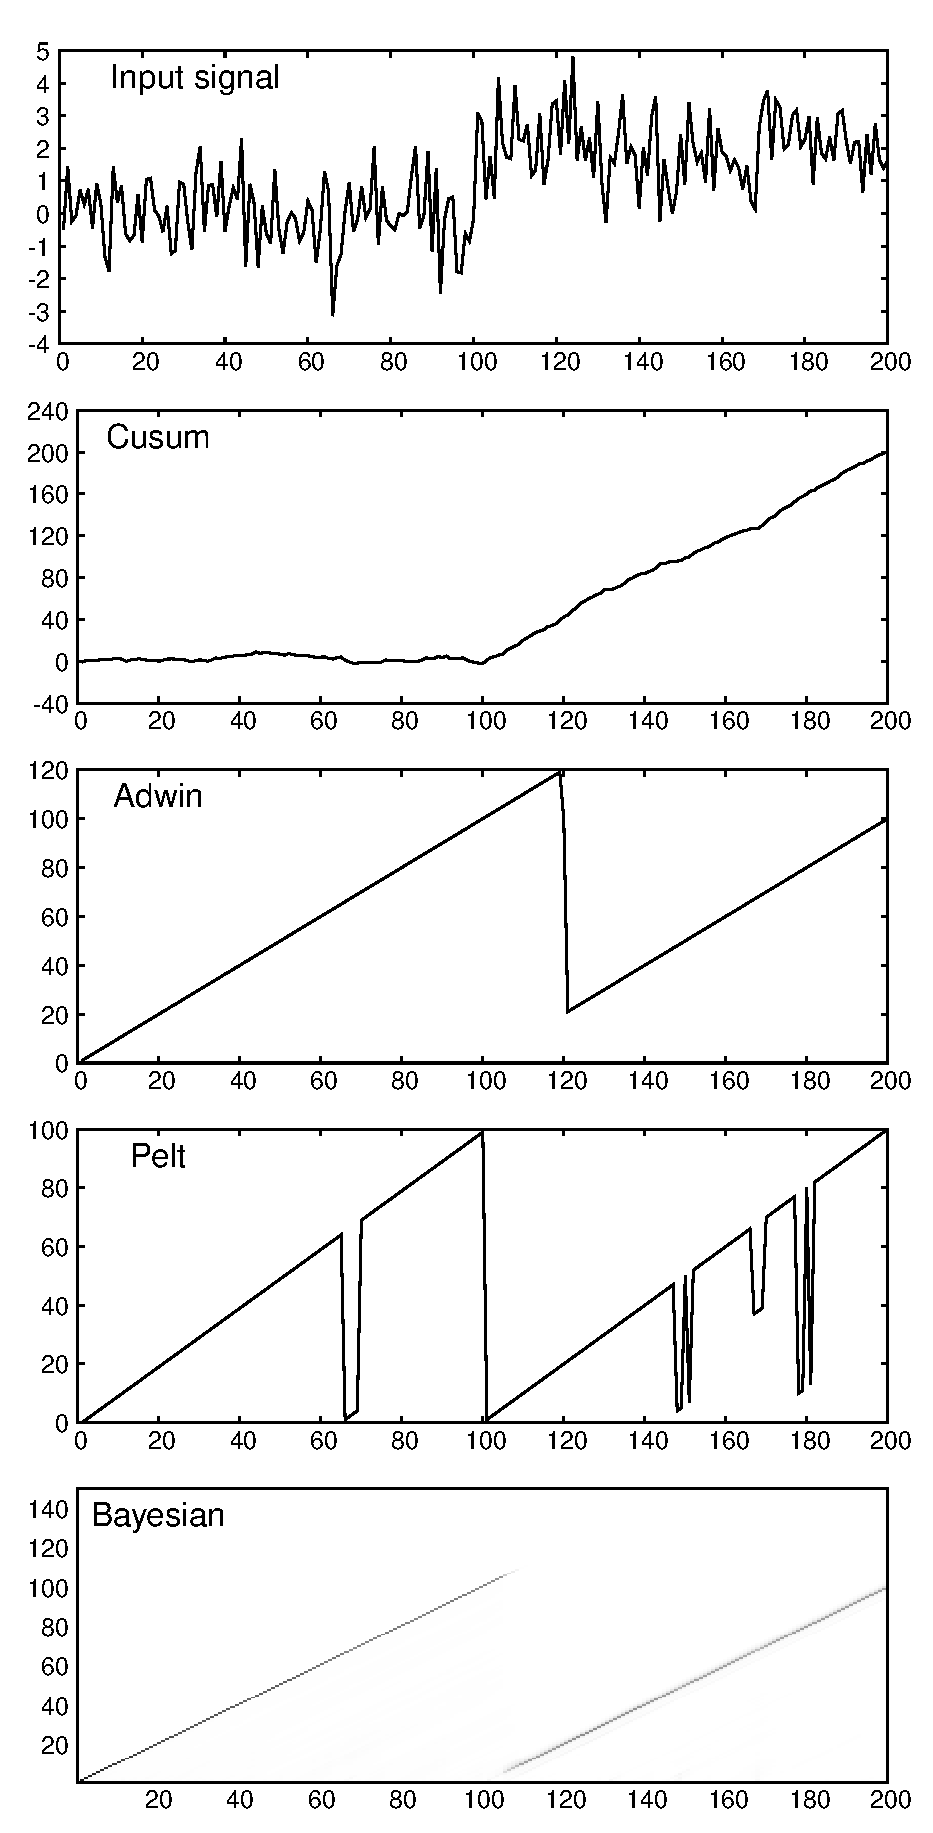
\includegraphics[height=0.9\textwidth]{images_gnu/detectors_output_stats}
	\caption{All}\label{fig:all_detectors_stats}
\end{figure}

\section{Adwin}

\begin{figure}[!htb]
	\centering
	\includegraphics[width=0.9\textwidth]{images/example_output_adwin.eps}
	\caption{ADWIN}\label{fig:adwin_output_example}
\end{figure}

\section{PELT method}
Offline detector used in online settings in ~\cite{marrero2013aclac}.
~\cite{killick2012optimal}
Pelt method is based on a common approach of  minimising a cost function over possible numbers and locations of change points.
Pelt is based on~\cite{jackson2005algorithm}, but involves a pruning step reducing the computational cost but not affecting exactness of the resulting segmentation.
Dynamic programming~\cite{bellman1966dynamic}.

Time interval $I$.
Ordered sequence of data $y_{1:n}=(x_1,\dots,y_n)$.
A partition $P$ of an interval $I$ is a set of blocks is defined  by change points $\tau_{1:m}=(\tau_1, \dots, \tau_m)$.
Each change point is an integer between 1 and $n-1$.
We define $\tau_0=0$ and $\tau_{m+1}=n$.
$m$ change points split the data into $m+1$ segments, $i$-th segment is $y_{\tau_{i-1} : \tau_i}$.
For example, if there is one changepoint $\tau_1$ the segments are $B_1=y_{\tau_0:\tau_1}$ and $B_2=y_{\tau_1:\tau_2}$ where $\tau_2 \equiv n$.
The goal is to find an optimal partition by minimising the cost function defined by Equation\ref{eq:cost_function}
\begin{equation}\label{eq:cost_function}
	\sum_{i=1}^{m+1} [ C(B_i) ] + \beta f(m),\: \text{where } B_i \equiv y_{\tau_{i-1} : \tau_i}
\end{equation}
where $\beta f(m)$ is a regularization term to prevent overfitting.
Commonly used cost functions are twice the negative log likelihood~\cite{guyon1999underfitting,chen2011parametric},
quadratic loss and cumulative sums~\cite{inclan1994use, rigaill2010pruned}. 
The most common choices for the regularization term are usually $\beta f(m) = \beta m$.
Examples are Akaike's Information Criterion (AIC\cite{akaike1974new}) $\beta=2p$ and Schwartz Information Criterion (BIC\cite{schwarz1978estimating}) ($\beta = p \log{n}$) where $p$ is the number of additional parameters introduced by adding a new changepoint.
Dynamic programming optimal segmentation is based on the next principle of optimality
\begin{theorem}
Let $P^{\text{max}}$ be an optimal optimal partition of $I$
\end{theorem}	

\begin{algorithm}[!h]
	\begin{algorithmic}
		\Function{pelt}{$Y$, $\sigma$, $C(s,t)$}
		\State n = length($Y$)
		\State $F$ = zeros(n)\Comment{Optimal segmentation costs till $t$}
		\State $F[0] = - \log(n)$
		\State previous\_changes\_opt = zeros[n]\Comment{Optimal previous change location}
		\For{t $\in$ [2, n]}
		    \State previous\_changes\_possible = $1,\dots,t-1$
		    \State i = 0
		    \For{s $\in$ previous\_changes\_possible}
		         \State i += 1
		        \State segmentation\_costs[i] = $C(s, t)$
		    \EndFor
		    \State costs = $F[\text{previous\_changes\_possible}]$ + segmentation\_costs + $\log(n)$
		    \State $F[t+1] = min(\text{costs})$
		    \State $\text{previous\_changes\_opt}[t] = \text{previous\_changes\_possible}[argmin(\text{costs})]$
		\EndFor
		\State detections = $\text{fn\_extract\_detections(previous\_changes\_opt)}$
		\EndFunction
	\end{algorithmic}
\end{algorithm}

\begin{figure}[!htb]
	\centering
	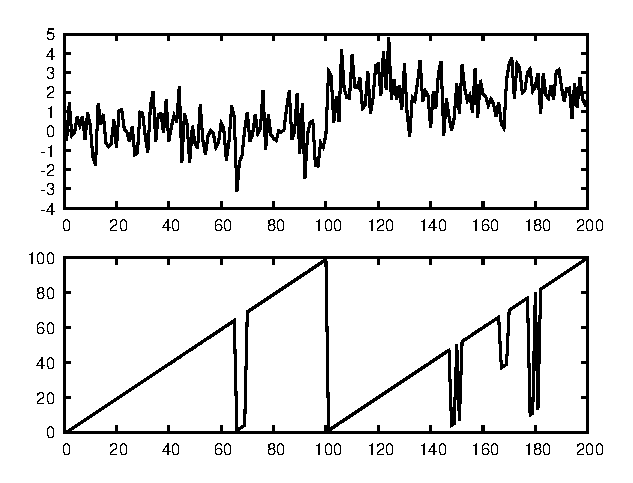
\includegraphics[width=0.9\textwidth]{images/example_output_pelt.eps}
	\caption{PELT}\label{fig:pelt_output_example}
\end{figure}


\section{Bayesian detector}
\cite{adams2007bayesian}
BD detector works by recursively estimating posterior probability distribution $P(r_t | \pmb{x}_{1:t}, \theta)$ of the \textit{run length} variable $r_t$ which is a time since the last changepoint.
Changepoint is an event when
\begin{equation}
	\operatorname*{arg\,max}_{r_t} P(r_t | \pmb{x}_{1:t}, \theta) = 0
\end{equation}
%\[\]
%$r_t = 0$
Every time a new measurement $x_t$ is observed the \textit{posterior} distribution is recalculated using the Bayes` theorem to update parameters of the distributions used to model data
\[
(r_t | \pmb{x}_{1:t}) = \frac{P(r_t, \pmb{x}_{1:t})}{P(\pmb{x}_{1:t})}
\]
and the law of total probability
%$P(x) = \sum_{y} P(x|y) p(y)$
\begin{equation}
	P(r_t|\:\LargeCdot) = \sum_{r_{t-1}} P(r_{t} | \: r_{t-1},\:\LargeCdot) \: P(r_{t-1}|\:\LargeCdot)
\end{equation}
to take into account values from all the runs in the past.
The \textit{prior} probability of the change $P(r_t=0|t)$ in BD detector is specified using the constant-value hazard rate $h$ which is a prior probability to observe a change and which is supposed to be known before the change detection process starts.
\begin{figure}[!htb]
	\centering
	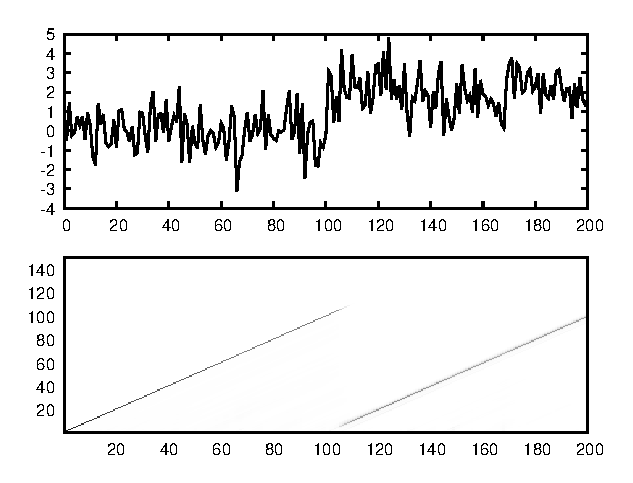
\includegraphics[width=0.9\textwidth]{images/example_output_bayes.eps}
	\caption{Bayes}\label{fig:bayes_output_example}
\end{figure}

\section{CUSUM detector}
In this section, we describe the CuSum~\cite{Page1954} detector and its output statistic properties important for measuring performance metrics in static and dynamic settings.
Changes in the stream of measurements reflect dynamics of observed phenomenon happening in time.
Therefore, strictly speaking, any change is a gradual process.
In this paper, for simplicity, we refer to change points and to detections as individual time moments as if change would have happen instantly. If change is gradual and spans time interval then it can be reduced to a single time moment by considering the start or end of the change event~\footnote{Gradual change may become represented as an abrupt change in the time series also due to the sampling rate of measurements}. 
Change points in the signal are characterized by the time moment when they happened and by the corresponding mean shift value in the signal.
\begin{definition}
	Change point is a time moment $t^c$ when statistical properties of the data stream change significantly accordingly to a predefined criteria.
\end{definition}
\begin{definition}
	Detection is a time moment $t^d$ when a detector alarms a change.
\end{definition}
For example, if $x_i \sim \mathbb{N}(\mu_1, \sigma)$ for $i < k$ and $x_i \sim \mathbb{N}(\mu_2, \sigma)$ for $i \geq k$,
then we say that a change point occurred at time moment $t_k$, i.e. $t^{\text{c}}_{k} \equiv t_k$.
In general, detection can usually be alarmed before or after a change point.
If $t^{\text{d}}_k > t^{\text{c}}_k$, then change is detected with the delay $t^{\text{d}}_k - t^{\text{c}}_k$.
%TOMMI: Can we give definition like below? I.e. to say that ALL too-early alarms are false alarms?
If $t^{\text{d}}_k < t^{\text{c}}_k$ then detection $t^{\text{d}}_k$ is a false alarm (FA).

As an input, CuSum detector receives time series of observations~\ref{eq:input_ts} usually taken at constant sampling rate.
\begin{equation}\label{eq:input_ts}
	(x_i)_{i=1}^{N} \equiv (x_1, x_2, \dots, x_N)
\end{equation}
taken at corresponding time moments $(t_i)_{i=1}^N$.
Observations and time moments are enumerated by index $i$ mapping $t_i$ to observations $x_i$ and vice versa.
CuSum works through a sequential calculation of the output statistic as follows
% Cusum rule: https://www.itl.nist.gov/div898/handbook/pmc/section3/pmc323.htm
\begin{align}
	S_0 &= 0 \nonumber \\
	S_{n} &= \max (0, S_{n-1} + x_n - \mu_0 - k )\label{eq:cusum_scheme}.
\end{align}
% Detections are alarmed at time moments when Cusum's output statistic exceeds a threshold value $h$.
Detections are alarmed at time moments when $S_{t+1} > h$, i.e. when output statistic exceeds a threshold value $h$.
In \eqref{eq:cusum_scheme}, $\mu_0$ is the estimate of the in-control state signals' mean value.
The parameter $k$ is called allowance value and it depends on the level of mean shift $\delta=\mu_2-\mu_1$ that we aim to detect.
\begin{figure}[!htb]
	\centering
	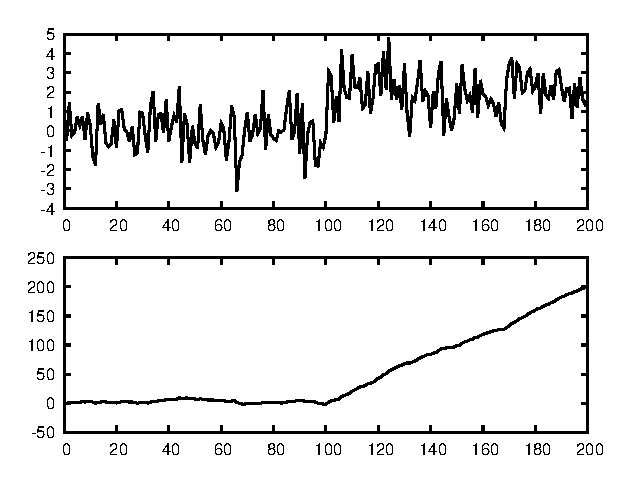
\includegraphics[width=0.9\textwidth]{images/example_output_cusum.eps}
	\caption{CuSum}\label{fig:cusum_output_example}
\end{figure}

%===============================================================================%
%                               RECURRENCY
%===============================================================================%
\chapter{Predictability And Recurrency}
Adaptive learning in concept drift.
Predictability of events in the data stream.
~\cite{feller2008introduction}
Sums of independent random variables.
Recurrency is a form of predictability.

\section{Inter-arrival times modeling}
Commonly used probability distributions for modelling inter-arrival times.


\chapter{Main results}
~\cite{MaslovSDM2016, MaslovIJCNN2017}

\section{Pccf}~\label{sec:pccf}
If change points are expected to reoccur in the input signal, then this prior information can be used to approximate prediction time intervals, or regions of interest (ROI), where changes are most likely to appear in the future.
Once calculated, and if predictions are correct, then this information can further be used to reduce the false alarm rate of the change detection process, %at the least
and potentially to reduce detection delays too.
FA rate can be decreased just by disregarding detections outside prediction intervals, and the detection delay can be decreased by increasing sensitivity of the detector within prediction intervals.
But, as mentioned, if sensitivity is increased, then probability of FA events will also  increase.
Possibility of decreasing detection delays in the presence of prediction interval is a subject of Experiments section.
We describe next how to calculate prediction intervals for reoccurring change points.

To calculate ROIs for recurrent change points we use a prediction confidence change function (Pccf) proposed in our previous work~\cite{MaslovSDM2016}, where it was calculated using convolutions.
Below we calculate Pccf for several commonly used distributions of inter-arrival times values using moment generating functions, what is a more concise way than when using convolutions.
%~\footnote{we useterms recurrent and reoccurring interchangebly}
% The difference to the previous work is that we calculate Pccf in a concise
% way using moment generating functions and we calculate it for several
% commonly used distributions used for inter arrival time modelling.
%In our previous work we applied threshold value to the calculated probability estimates, but now we found it much more practical just to use equally spaced time moments surrounded by time intervals of a fixed size.
% Probability estimates given by Pccf should be used to assess confidence intervals for predictions and for assessment of how many changes in the future we want to make a prediction for.
Let's start with definitions.
\begin{definition}
	Change points $t_i^{\text{c}}$ are recurrent if their inter-arrival times $t_{i}^{c} - t_{i-1}^{c}$
	% \begin{equation}\label{eq:recurrence_relation}
	%     \Delta_i = t_{i}^{c} - t_{i-1}^{c}
	% \end{equation}
	are i.i.d.\ from the same probability distribution.
	E.g., $t_{i}^{c} - t_{i-1}^{c} \sim \mathbb{N}(\mu, \sigma)$ if $\sigma$ is small.
\end{definition}
%The recurrence relation for recurrent changes is
%\begin{equation} x_{n+1} = x_n + \delta_n \end{equation}
%
Pccf function value at time moment $t_i$ is a probability estimator of recurrent change point to occur at this time moment.
%Pccf function value at time moment $t_i$ is a probability estimation of the event of observing recurrent changepoint at this moment.
%Recurrent changepoints form a sequence determined by recurrence relation given by Equation~\ref{eq:recurrence_relation}.
% $t_{i}^{\text{CHP}} = t_{i-1}^{\text{CHP}} + \Delta_i$.
Pccf can be represented as a matrix~\ref{eq:pccf_matrix} in which elements at row $k$ and column $i$ are probability estimates for change point $t_k^{\text{c}}$ to appear at time moment $t_i$.
\begin{equation}~\label{eq:pccf_matrix}
	\text{PCCF}_{k,i} \equiv P(t_{k}^{\text{c}} = t_i) % \: \forall \:  k, i \in [1,\dots,N
\end{equation}
When calculating ROIs we are interested in total probability of any changepoint occurring at every time moment within prediction horizon.
Since events $t_k^{\text{c}} = t_i$ are disjoint we need to sum up rows of the matrix $\text{PCCF}_{k,i}$
\begin{equation}~\label{eq:pccf_vector}
	\text{PCCF}_{i \in 1:N} = \sum_{k=1}^{N} P(t_k^{\text{c}} = t_i) \equiv \sum_{k=1}^{N} \text{PCCF}_{k,i}
\end{equation}
Further by Pccf we call the vector given by Equation~\ref{eq:pccf_vector}.
%, i.e.  $\sum_{k=1}^{N} P(t_k^{\text{CHP}} = t_i)$.
%	\begin{equation}
%		\text{Any } t_{k}^{\text{CHP}} = t_i
%		% \text{ or } t_{2}^{\text{CHP}} = t   \dots t_{k}^{\text{CHP}} = t
%		%C_1 = t \text{ or } C_2 = t \text{ or } \dots C_n = t
%		\label{eq:events_union}
%	\end{equation}
%Since events $t_k^{\text{CHP}} = t_i$ are disjoint Pccf can be calculated as
%\begin{equation}
%	\sum_{i=1}^{N} \sum_{k=1}^{N} P(t_k^{\text{CHP}} = t_i).
%\end{equation}
%\begin{equation}
%	P\Big(\bigcup\limits_{k=1}^{N} (t_k^{\text{CHP}} = t_i) \Big ) = \sum_{k=1}^{N} P(t_k^{\text{CHP}} = t_i)
%\end{equation} % Wasserman, page5

The sum~\ref{eq:pccf_vector} can be calculated using the notion of moment generating function (Mgf).
As an example, let's assume a Gaussian distribution for inter-arrival times, i.e. $t_{i}^{\text{c}} - t_{i-1}^{\text{c}} \sim \mathbb{N}(\mu, \sigma)$,
with $\sigma$ small enough so that every next change can not happen before the previous one.
For example, if $\mu=60$ seconds and standard deviation is $\sigma=5$ seconds then, using Chebyshev's inequality~\ref{eq:chebyshev_ineq}, probability of
$\mathbb{P}(|t_{i}^{\text{c}} - t_{i-1}^{\text{c}}| \geq 60) \leq 0.007$.
\begin{equation}\label{eq:chebyshev_ineq}
	\mathbb{P}(|X-\mu| \geq k \sigma) \leq \frac{1}{k^2} % %\mathbb{P}(|X-\mu| \geq t) \leq \frac{\sigma^2}{t^2}
\end{equation}
%\subsec{Predicting sequential events}
% Resources
% \href{https://www.youtube.com/playlist?list=PL2SOU6wwxB0uwwH80KTQ6ht66KWxbzTIo}{Statistics 110: Probability}
%- [lec24] [Lecture 24: Gamma distribution and Poisson process](https://www.youtube.com/watch?v=Qjeswpm0cWY&index=24&list=PL2SOU6wwxB0uwwH80KTQ6ht66KWxbzTIo)
%- [lec22] [Lecture 22: Transformations and Convolutions](https://www.youtube.com/watch?v=yXwPUAIvFyg&list=PL2SOU6wwxB0uwwH80KTQ6ht66KWxbzTIo&index=22)
%- [lec17] [Lecture 17: Moment Generating Functions](https://www.youtube.com/watch?v=N8O6zd6vTZ8&index=17&list=PL2SOU6wwxB0uwwH80KTQ6ht66KWxbzTIo)
%- [lec18] [Lecture 18: Mgfs Continued](https://www.youtube.com/watch?v=tVDdx6xUOcs&list=PL2SOU6wwxB0uwwH80KTQ6ht66KWxbzTIo&index=18)
%- [math.tntech.edu: Sum of independent random variables](http://math.tntech.edu/ISR/Introduction_to_Probability/Distributions_of_Functions/thispage/newnode11.html)
%- [Table of Common Distributions](http://www.stat.tamu.edu/~twehrly/611/distab.pdf) taken from Statistical Inference by Casella and Berger
%The sum~\ref{eq:pccf_sum} can be calculated by calculating Mgf of the sum of i.i.d.\ variables and after that by pattern\ - similarity to the Mgf of individual variable find the PDF of the sum.
%\begin{definition}
By definition, Mgf, or Laplace transform, of random variable $X$ is~\ref{eq:mgf}
%~\footnote{Mgf is $\mathbb{E}(e^{tX})$ while characteristic function is $\mathbb{E}(e^{i t X})$.}
\begin{equation}\label{eq:mgf}
	M_{X}(t) = \mathbb{E}(e^{t X}), \: t \in \mathbb{R}
\end{equation}
%\begin{equation}~\label{eq:mgf}
%	%\psi_{X}(t) = \mathbb{E}(e^{t X}) = \int e^{tX} d F(x)
%	M_{X}(t) = \mathbb{E}(e^{t X})
%\end{equation}
% Moments of a distribution is computed as $\psi^{(k)} (0)=\mathbb{E}(X^k)$.
% Mgfs is a convenient tool to obtain distribution of sums of random variables.
Using the property that expected value of the product of two independent random variables is the product of their expected values $\mathbb{E}(X \dot Y)=\mathbb{E}(X)\mathbb{E}(Y)$, Mgf of the sum of independent random variables is a product of individual Mgfs (Equation~\ref{eq:mgf_of_sum}).
\begin{equation}\label{eq:mgf_of_sum}
	M_{X+Y}(t) = \mathbb{E}(e^{t (X+Y)}) = \mathbb{E}(e^{t X}) \mathbb{E} (e^{t Y}) \equiv M_{X}(t) M_{Y}(t)
\end{equation}
For the Gaussian distribution Mgf is $\exp{(\mu t + \frac{\sigma^2 t^2}{2})}$ and therefore
\begin{equation}\label{eq:mgf_gauss}
	M_{X+Y}^{\text{Gaussian}}(t)  = \exp \Big ((\mu_X + \mu_Y) t + \frac{(\sigma_X^2 + \sigma_Y^2) t^2}{2} \Big )
	% M_{X+Y}^{\text{Gaussian}}(t)  = \exp \Big [ (\mu_X + \mu_Y) t + \frac{(\sigma_X^2 + \sigma_Y^2) t^2}{2} \Big ]
\end{equation}
But~\ref{eq:mgf_gauss} is Mgf of the Gaussian distribution with parameters $\mu=\mu_1+\mu_2$ and $\sigma=\sqrt{\sigma_X^2 + \sigma_Y^2})$.
Therefore if probability distribution of the first change point is $t_1^{\text{c}} \sim \mathbb{N}(\mu, \sigma)$ then $t_2^{\text{c}} \sim \mathbb{N}(2\mu, \sigma \sqrt{2})$, etc.
And Pccf is a sum~\ref{eq:pccf_gaussian}
\begin{equation}\label{eq:pccf_gaussian}
	\text{PCCF}^{\text{Gaussian}} \equiv \sum_{k=1}^N \mathbb{N}(k \mu, \sqrt{k} \sigma)
\end{equation}
% Mgfs for commonly used for inter-arrival times modelling distributions are~\cite{wasserman2013all}
% as follows.
% for Exponential distribution with rate $\lambda$ it is $\frac{\lambda}{\lambda - t}$;
% and for the Gamma distribution $\Gamma(\alpha, \lambda)$ is $\Big ( \frac{1}{1- \lambda t} \Big )^{\alpha}$.
% $\Big (\frac{\lambda}{\lambda - t} \Big)^{\alpha}$ %([ref](http://math.tntech.edu/ISR/Introduction_to_Probability/Distributions_of_Functions/thispage/newnode11.html))
%
% % POSISSON is not needed, as we model inter-arrival times, not number of occurences
%\item Poisson is $e^{\lambda (e^t-1)}$
%
% $\mathbb{E}(e^{tX}) = \sum_{k=0}^{\infty} e^{tk} e^{-\lambda} \lambda^k/k! = e^{\lambda (e^t-1)}$
% https://en.wikipedia.org/wiki/Gamma_distribution#Summation
% https://stats.stackexchange.com/questions/51605/the-sum-of-two-independent-gamma-random-variables
% proof: https://en.wikipedia.org/wiki/Characteristic_function_%28probability_theory%29#Example
%Proof for the Gamma can be found \href{https://en.wikipedia.org/wiki/Characteristic\_function\_\%28probability\_theory\%29#Example}{here}. Characteristic functions are $\phi_X(t)=(1-\lambda i t)^{-a}$ and $\phi_Y(t)=(1-\lambda i t)^{-b}$. Therefore $\phi_{X+Y}(t) = (1-\lambda i t)^{-(a+b)}$.
%
% Poisson & $\mathbb{E}(e^{tX}) = \sum_{k=0}^{\infty} e^{tk} e^{-\lambda} \lambda^k/k! = e^{\lambda (e^t-1)}$ & Inter-arr. times are from Exp. And Pdf is for Gamma \\
%Weibull? & & p pp\\
% Gamma~\cite{wasserman2013all}
%
%  Corresponding Mgfs for the sums are as follows.
%  for Gamma distribution $M_{X+Y} (t) =  \Big (\frac{\lambda}{\lambda - t} \Big)^{a + b}$
%  and for Exponential distribution is $\frac{\lambda}{\lambda-t}$.
%
%  Gaussian,
%  If $X \sim N(\mu_X, \sigma_X)$ and $Y \sim N(\mu_Y,\sigma_Y)$ then $X+Y \sim N(\mu_X + \mu_Y, \sqrt{\sigma_X + \sigma_Y})$
%  $$M_{X+Y}(t) = \exp \Big ( t \mu_X  + \frac{\sigma_X^2 t^2}{2} \Big) \cdot \exp \Big ( t \mu_Y  + \frac{\sigma_Y^2 t^2}{2} \Big) = \exp \Big [ (\mu_X + \mu_Y) t + \frac{(\sigma_X^2 + \sigma_Y^2) t^2}{2} \Big ] $$ which is a characteristic function of the normal distribution with parameters $\mu =  \mu_X + \mu_Y$ and $ \sigma^2 = \sigma_X^2 + \sigma_Y^2$.
%
%
% $\Gamma(k, \lambda)$.
% Copied to for)thesis.tex
%
%\begin{itemize}
%	% POSISSON is not needed, as we model inter-arrival times, not number of occurences
%	%    %\item \textbf{For the Poisson.}
%	%$$M^P_{X+Y} (t) =  e^{\lambda (e^t-1)}  e^{\mu (e^t-1)} =  e^{(\lambda+\mu) (e^t-1)}$$
%	%It means $X+Y \sim \text{Poiss}(\lambda + \mu)$ (note: the sum of two Poissons is also a Poisson, which is not general for any distribution)
%	\item \textbf{Gaussian}
%	If $X \sim N(\mu_X, \sigma_X)$ and $Y \sim N(\mu_Y,\sigma_Y)$ then $X+Y \sim N(\mu_X + \mu_Y, \sqrt{\sigma_X + \sigma_Y})$
%	$$M_{X+Y}(t) = \exp \Big ( t \mu_X  + \frac{\sigma_X^2 t^2}{2} \Big) \cdot \exp \Big ( t \mu_Y  + \frac{\sigma_Y^2 t^2}{2} \Big) = \exp \Big [ (\mu_X + \mu_Y) t + \frac{(\sigma_X^2 + \sigma_Y^2) t^2}{2} \Big ] $$
%
%	which is a characteristic function of the normal distribution with parameters $(\mu =  \mu_X + \mu_Y, \sigma^2 = \sigma_X^2 + \sigma_Y^2)$.
%
%	\item \textbf{Gamma}
%	If $X \sim \Gamma(a, \lambda), Y \sim \Gamma(b, \lambda)$ then $X+Y \sim \Gamma(a+b, \lambda)$.
%
%	$$M_{X+Y} (t) = M_X (t) \cdot M_Y (t) = \Big (\frac{\lambda}{\lambda - t} \Big)^{a}  \Big (\frac{\lambda}{\lambda - t} \Big)^{b} =  \Big (\frac{\lambda}{\lambda - t} \Big)^{a + b}$$
%
%	\item \textbf{Exponential}
%	Mgf for the exponential distribution with $\lambda=1$ is $\frac{1}{1-t}$ where $t<1$.
%	% Lec.14 (Statistics 101): https://www.youtube.com/watch?v=Qjeswpm0cWY&index=24&list=PL2SOU6wwxB0uwwH80KTQ6ht66KWxbzTIo
%	% START: 23:27
%	% Using the property of moment generating functions (by definition)
%	% \[\psi_{X+Y}(t) = \mathbb{E}(e^{t (X+Y)}) = \mathbb{E}(e^{t X}) \mathbb{E} (e^{t Y})\]
%	Mgf for the $n$-th event $T_n = \sum_{j=1}^{n} X_j, \text{ where } X_j \sim e^{-\lambda t}$ is $\Big ( \frac{1}{1-t} \Big )^n$.
%	But Mgf for $Y \sim \Gamma(n,1)$ is also $\Big(\frac{1}{1-t} \Big)^n$.
%	Therefore if inter-arrival times are i.i.d. from the exponential distribution with parameter $\lambda$ the PDF for the k-th event is $\Gamma(k, \lambda)$.
%	%\begin{equation}
%	%    \mathbb{E}(e^{tY}) = \frac{1}{\Gamma(n)} \int_{0}^{\infty} e^{ty} y^{n} e^{-y} \frac{d y}{y} = \frac{1}{\Gamma(n)} \int_{0}^{\infty} y^n e^{-(1-t)y} \frac{d y}{y}
%	%\end{equation}
%	%Let, $x=(1-t)y$, then $d x = (1-t) d y$, then we get
%	%\begin{equation}
%	%    \mathbb{E}(e^{tY}) = \frac{(1-t)^{-n}}{\Gamma(n)} \int_{0}^{\infty} x^n e^{-x} \frac{d x}{x} = \Big(\frac{1}{1-t} \Big)^n
%	%    \label{eq:mgf_gamma_1}
%	%\end{equation}
%	%This is (Equation~\ref{eq:mgf_gamma_1}) the same Mgf as Mgf for the sum of i.i.d. from Exponential distribution with $\lambda=1$ (Equation~\ref{eq:mgf_exp_n}).
%
%	%If $X \sim Exp(\lambda_1)$ and $Y \sim Exp(\lambda_2)$ then $X+Y \sim $
%	%$$M^E_{X+Y}(t) = \frac{\lambda_1}{\lambda_1 - t} \frac{\lambda_2}{\lambda_2 - t}$$
%\end{itemize}

Using the same logic it is straightforward to calculate Pccfs for Exponential and Gamma distributions (Table~\ref{table:pccfs}).
\begin{table}[!htb] \caption{Pdf's for distributions of inter-arrival times.}\label{table:pccfs}
	\begin{center}
		\begin{tabular}{|l|l|c|c|}
			\hline
			Distribution & Mgf & PDF of the $k$-th event & PCCF  \\[5pt]
			\hline
			Gaussian & $\exp{ (\mu t + \frac{\sigma^2 t^2}{2}) }$ & $\mathcal{N}(k \mu, \sqrt{k} \sigma)$ & $\sum_{k=1}^N \mathcal{N}(k \mu, \sqrt{k} \sigma)$ \\
			Gamma $\Gamma(\alpha, \lambda)$ & $\Big ( \frac{1}{1- \lambda t} \Big )^{\alpha}$ & $\Gamma(k \alpha, \lambda)$ & $\sum_{k=1}^N \Gamma(k \alpha, \lambda)$\\
			Exponential & $\frac{\lambda}{\lambda - t}$ & $\Gamma(k, \lambda)$ & $\sum_{k=1}^N \Gamma(k, \lambda)$\\
			\hline
		\end{tabular}
	\end{center}
\end{table}
%In the paper~\cite{MaslovSDM2016} we considered a Gaussian distribution instead of, for example, Gamma distribution assuming that standard deviation ``$\sigma$ is small enough'' so that we can neglect probabilities of the events in the negative values tail of the distribution.
%Markov's inequality.63~\cite{wasserman2013all}.p.249~\cite{feller2008introduction}: if $X$ is a non-negative random variable, then $\forall t >0$
%\begin{equation}
%	\mathbb{P}(X>t) \leq \frac{\mathbb{E}(X)}{t}
%	\label{eq:markov_ineq}
%\end{equation}
%Chebyshev's inequality: let $\mu=\mathbb{E}(X)$ and $\sigma^2=\mathbb{V}(X)$ then,
Figure~\ref{fig:pccf_example} depicts Gaussian Pccf.
Prediction intervals (ROI) can be calculated by applying a threshold value for Pccf and then ROIs will be determined by time moments when Pccf exceeds this threshold.
In this way we would take into account uncertainty in the predictions for $k$-th change points which will increase as $\sqrt{k} \sigma$ (Equation~\ref{eq:pccf_gaussian}).
Another way is to use the property that Pccf extremums are equally spaced (Equation~\ref{eq:rois})~\cite{MaslovSDM2016} by time intervals $\mu$.
After estimating $\mu$ between changes and choosing the number of change points $k$ to predict and ROIs width prediction interval are determined by Equation~\ref{eq:rois}.
\begin{equation}\label{eq:rois}
	\text{ROI}s = (\mu \pm \text{ROI}_{\text{Width}}, 2 \mu \pm \text{ROI}_{\text{Width}}, \dots , k \mu \pm \text{ROI}_{\text{Width}}).
\end{equation}
%\begin{figure}[htb!]
%	\centering
%	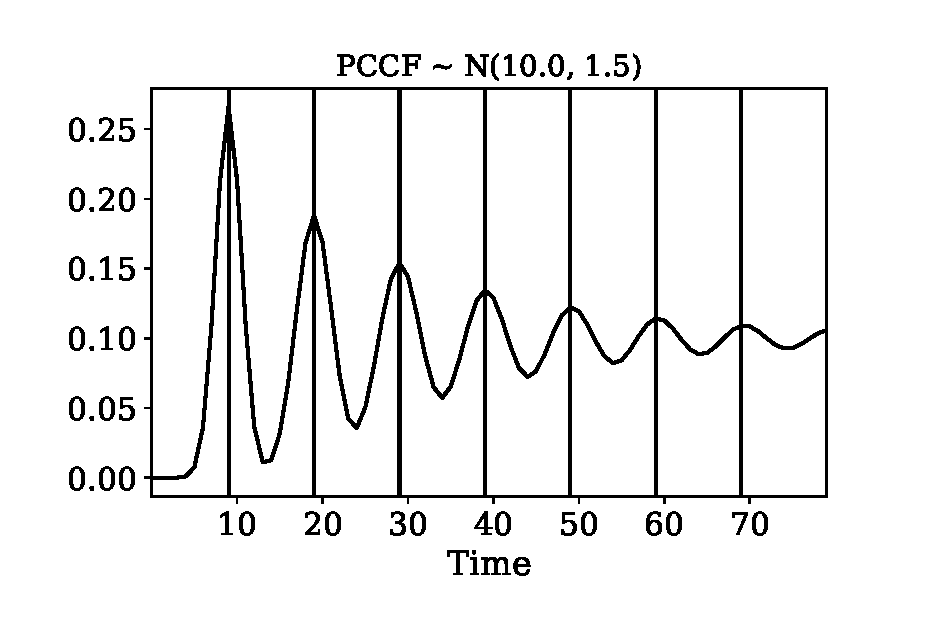
\includegraphics[scale=0.5]{img/pccf_example.eps}
%	\caption{
%		Gaussian PCCF.
%		The oscillating curve depicts probability estimation for the changepoint to occur at corresponding time moment.
%		Peaks are located at time moments $(\mu, 2 \mu, 3\mu, \dots)$.
%	}
%	\label{fig:pccf_example}
%\end{figure}
% Since Pccf decreases its values while oscillating and converging to the constant value over time we effectively choose first $k$ peaks of Pccf by applying threshold.
%By observing how fast Pccf converges to the constant level we can select $k$ based on visual inspection of Pccf behavior.
%Then we would need to select how many change points we need to predict
%After that ROI intervals can be allocated around Pccf's local extremums




\section{Integration with Bayesian detector}
\section{Integration with CuSum}

\chapter{MISC}
External~\cite{shewhart1931economic}
Included article~\cite{sha1}.
Concept drift and change detection problem.
Concept drift can be reduced to change detection in univariate time series?


\begin{itemize}
  \item Change detection:~\cite{basseville1993detection}
  \item Sequential change detection problem is a well studied problem, see for example in~\cite{tartakovsky2014sequential}, ~\cite{plasse2021streaming}. 

  \item Optimality of the change detection procedure was investigated in~\cite{Page1954},~\cite{Shiryaev2010,Shiryaev1961,Shiryaev1963}.
  Asymptotic and nonasymptotic optimality of cumulative sum algorithms was provedin~\cite{lorden1971procedures},~\cite{moustakides1986optimal},~\cite{moustakides2004optimality},~\cite{ritov1990decision}. In~\cite{Shiryaev1963,shiryaev2007optimal} the change point is modelled as a random variable with a known geometric distribution~\cite{veeravalli2014quickest} and optimal algorithm minimizing the average detection delay given constraint on the probability of false alarm is proposed. In our work we minimize the detection delay given a constraint on the maximum delay imposed by the prediction interval width. In~\cite{lorden1971procedures} asymptotic optimality of Cusum~\cite{Page1954} is proved according to the minimax criterion for delay with the mean time between false alarms going to infinity.

  \item Concept drift:
\end{itemize}

\chapter{Conclusion}

\tailmatter
\finnishsummary
Foo bar
%\inputencoding{utf8}
\bibliographystyle{plain}
\bibliography{references}
\appendices
\appendix{A}
\section{foobar}

\backmatter

\includedarticles
\begin{article}{sha1}
	\arttitle{Modelling Recurrent Events for Improving Online Change Detection}
	\artauthor{Alexandr Maslov, Mykola Pechenizkiy, Indr{\.e} {\v{Z}}liobait{\.e}, and Tommi K\"{a}rkk\"{a}inen}
	\artpublish{Proceedings of the 2016 SIAM International Conference on Data Mining}
	\artyear{2016}
	\artcopyright{XX}
	\artpages{1}
\end{article}
%
%\begin{article}{sha2}
%	\arthide
%	\arttitle{BLPA: Bayesian learn-predict-adjust method for online detection of recurrent changepoints}
%	\artauthor{Alexandr  Maslov, Mykola Pechenizkiy, Yulong  Pei, Indre {\v{Z}}liobait{\.e},  Alexander Shklyaev, Tommi Karkk{\"a}inen, and Hollm{\'e}n, Jaakko}
%	\artpublish{2017 International Joint Conference on Neural Networks (IJCNN)}
%	\artyear{2017}
%	\artcopyright{XXX}
%\end{article}

\printindex
\end{document}
